\chapter{Evaluation}
To ensure that the prototype satisfied our final problem statement, we had to evaluate our prototype through an usability and user experience combined test. 

\section{The usability test}
In order to find out to which degree our prototype met our usability and user experience requirements, we conducted a combined usability and user experience test

\subsection{Test goals}
The main goal of this test was to figure out if our target group perceived the prototype's usability and that the user experience was satisfaction. Although our original idea was that this test should be tested on our experts, unfortunately this was not possible which led us to test the prototype on regular students from AAU CPH, but in role as a garden designer and the customer.\\
Efficiency??\\
Learnability??\\
Safety???\\

\subsection{Sampling}
The combined usability test was conducted with the help of (number) participants. We used convenience sampling to find students at AAU CPH.

\subsection{Test specifics}
In \autoref{fig:test1} seen below, is the setup for our usability test.

\begin{figure}[H]
	\centering
	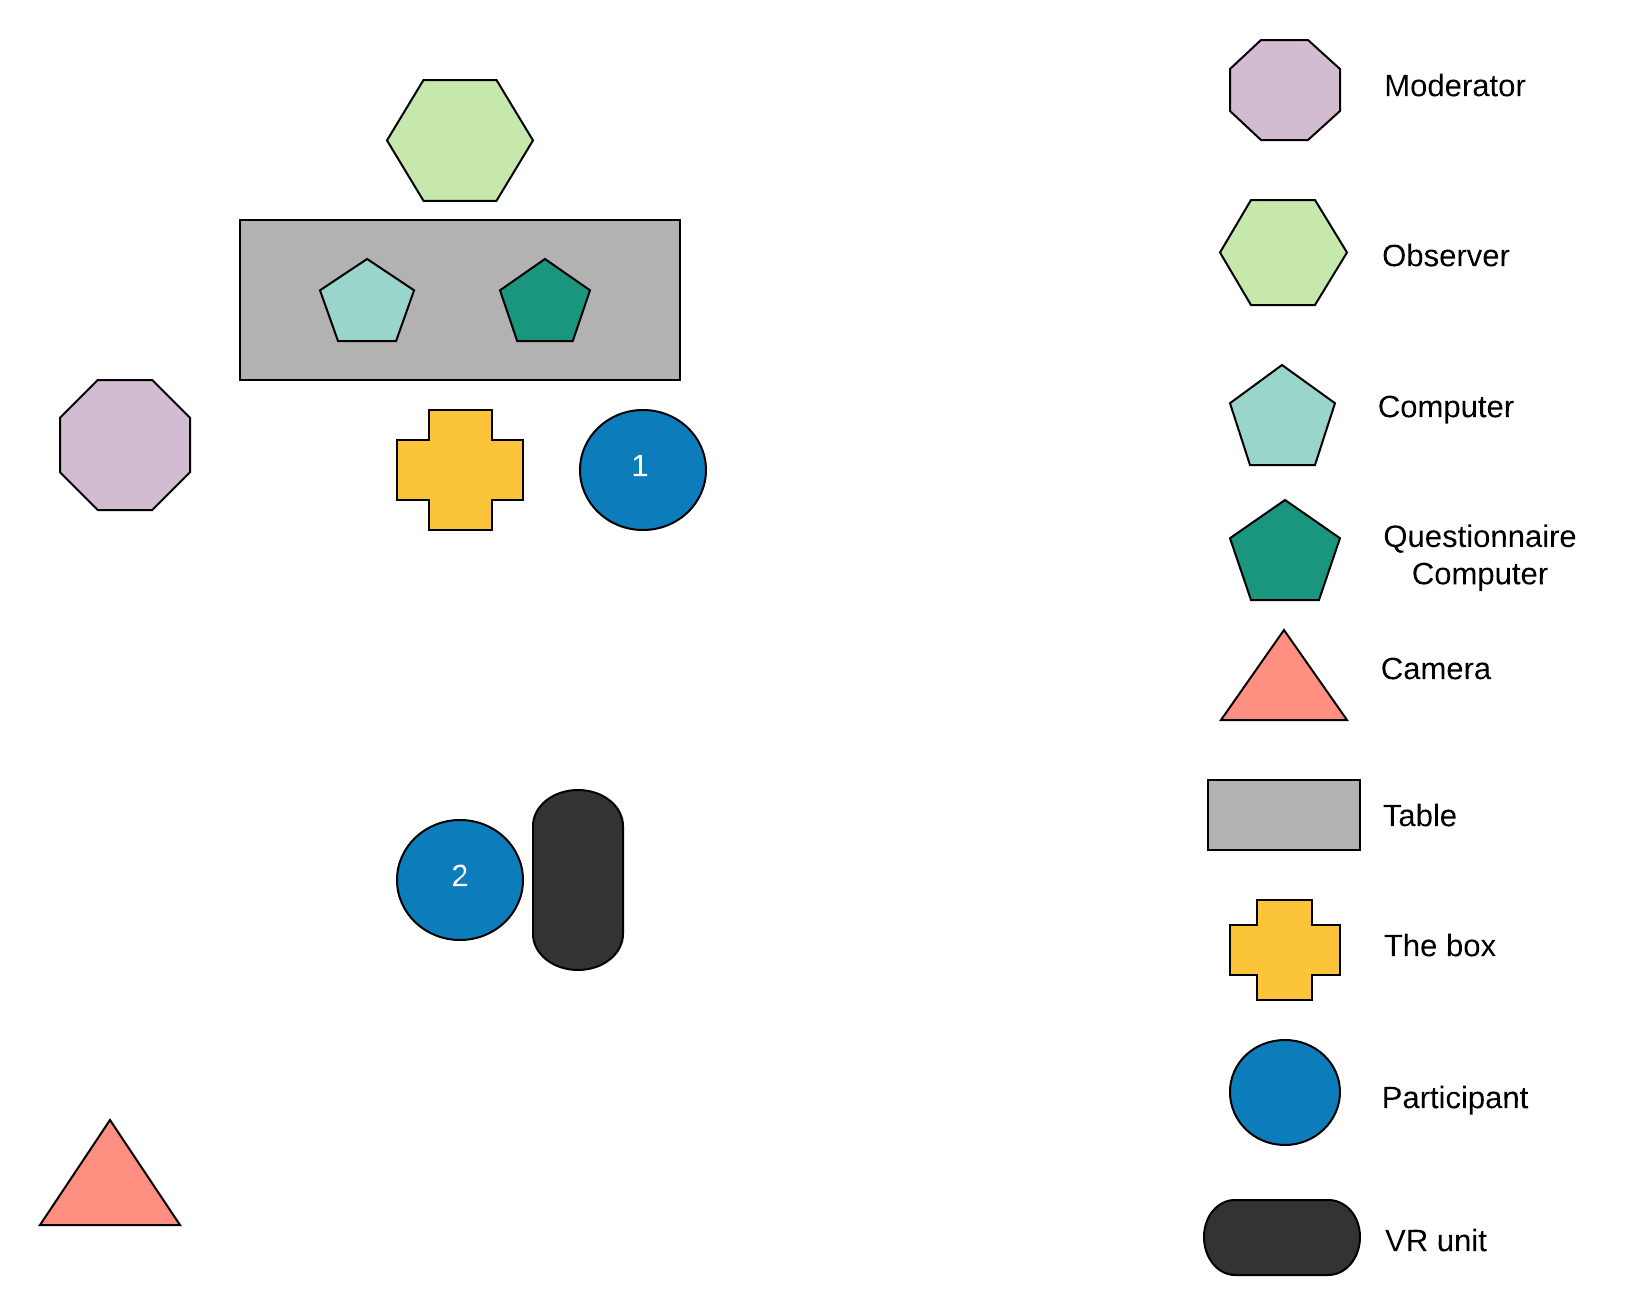
\includegraphics[width=1\linewidth]{figure/Evaluation/Test1.png}
	\caption{Our test setup, with the location of the participant, moderator, video camera and equipment. The two phases are visualized by the numbers in the circles.}
	\label{fig:test1}
\end{figure}

\subsection*{The equipment being used during the test}
\begin{itemize}
	\item[-] A camera running on a computer
	\item[-] The box where the tokens is placed with a camera inside
	\item[-] Laptop for filling out a questionnaire
	\item[-] HTC vive VR unit
\end{itemize}

\subsection*{Location and schedule}
The test took place Thursday 7/12 2017 in our group room at Aalborg University Copenhagen on Frederikskaj 12. Each testing with evaluation took approximately 15 to 20 minutes.

\subsection*{Test procedure}
Firstly, the participant was informed about the general purpose of the test, tasks and that they would give their consent to being filmed. After agreeing to this, the participant was asked to take the role of a client or an architect. Then they where asked to act like they needed a new garden and find out how the design should look. The client would take on the VR goggles and the architect would make a design with the markers with the help from the client. Afterwards the participants would switch roles and do the same thing again.

*Insert steps here*\\

After the participants tried their different roles they where asked to fill out a questionnaire (see appendix ??) as their respective roles, so each participant had to fill out two questionnaires. The questionnaires contained questions regarding the experience as a client and an architect.

\subsection{Results}
In this section we will display the results conducted from our questionnaires that the participants filled out after each role in the test (see \autoref{fig:boxPlotResults} and \autoref{fig:boxPlotResults2}). The questionnaires was not 100\% Likert scale questions, but we took those out and put them in a box plot. Some of the questions will be picked out and shown in a bar chart.
The questions is as follows:\\

Client Questions:\\
Rate the amount of discomfort you experienced during the test\\
Was the framerate (the frequency at which the screen updates) tolerable?\\
How engaged did you feel with the program?\\
How good did the environment and objects look?\\
Did you feel you had enough space to move around?\\
Could you easily communicate with the other participant?\\


\begin{figure}[H]
	\centering
\begin{tikzpicture}
\begin{axis}
[
boxplot/draw direction=y,
height=10cm,
width=15cm,
enlargelimits=0.03,
ytick={1,1.5,2,2.5,3,3.5,4,4.5,5},
xtick={1,2,3,4,5,6},
xlabel=Questions,
ylabel={Level of agreement},
xticklabels={
	1,2,3,4,5,6}
]
\addplot+[boxplot]
table[row sep=\\,y index=0] {
	data\\ 1\\ 1\\ 1\\ 2\\ 2\\ 2\\ 3\\ 4\\
};
\addplot+[boxplot]
table[row sep=\\,y index=0] {
	data\\ 2\\ 2\\ 2\\ 3\\ 4\\ 5\\ 5\\ 5\\
};   
\addplot+[boxplot]
table[row sep=\\,y index=0] {
	data\\ 4\\ 4\\ 4\\ 4\\ 4\\ 4\\ 4\\ 5\\ 
};   
\addplot+[boxplot]
table[row sep=\\,y index=0] {
	data\\ 2\\ 3\\ 4\\ 4\\ 4\\ 5\\ 5\\ 5\\
};  
\addplot+[boxplot]
table[row sep=\\,y index=0] {
	data\\ 2\\ 2\\ 3\\ 3\\ 3\\ 5\\ 5\\ 5\\
};  
\addplot+[boxplot]
table[row sep=\\,y index=0] {
	data\\ 1\\ 1\\ 4\\ 5\\ 5\\ 5\\ 5\\ 5\\
};  
 
\end{axis}
\end{tikzpicture}
\caption{Box plot graph showing the result of the client scale questions.}
\label{fig:boxPlotResults}
\end{figure}

Architect questions:\\
How easy was the product to use?\\
How easy was it to tell what the garden looked while you were building it?\\

\begin{figure}[H]
	\centering
\begin{tikzpicture}
\begin{axis}
[
boxplot/draw direction=y,
height=10cm,
width=15cm,
enlargelimits=0.03,
ytick={1,1.5,2,2.5,3,3.5,4,4.5,5},
xtick={1,2},
xlabel=Questions,
ylabel={Level of agreement},
xticklabels={
	1,2}
]
\addplot+[boxplot]
table[row sep=\\,y index=0] {
	data\\ 1\\ 3\\ 3\\ 4\\ 4\\ 5\\ 5\\ 5\\
};
\addplot+[boxplot]
table[row sep=\\,y index=0] {
	data\\ 1\\ 1\\ 2\\ 2\\ 2\\ 3\\ 3\\ 3\\
};   


\end{axis}
\end{tikzpicture}
\caption{Box plot graph showing the results of the architect Likert questions.}
\label{fig:boxPlotResults2}
\end{figure}

\begin{comment}
\begin{figure}[H]
	\centering
	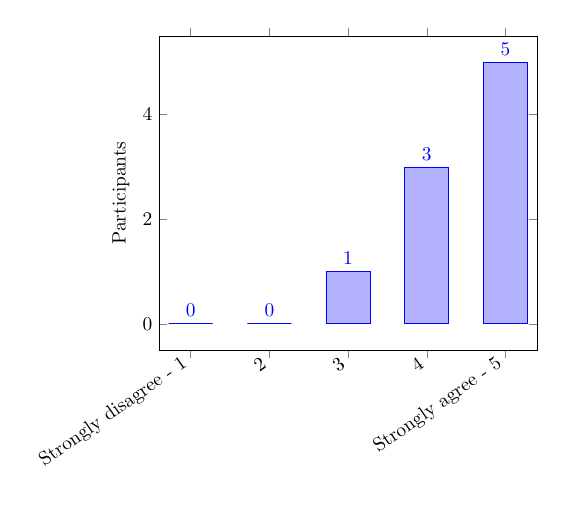
\begin{tikzpicture}[scale=0.7]
	\begin{axis}[ybar,bar width=0.8cm,enlargelimits=0.1,legend style={at={(0.5,-0.2)},anchor=north,legend columns=-1},ylabel={Participants},symbolic x coords={Strongly disagree - 1,2,3,4,Strongly agree - 5},xtick=data,nodes near coords,nodes near coords align={vertical},x tick label style={rotate=35,anchor=east},]
	\addplot coordinates {(Strongly disagree - 1,0) (2,0) (3,1) (4,3) (Strongly agree - 5,5)};
	\end{axis}
	
	\end{tikzpicture}
	\caption{Bar chart.}
	\label{fig:barChartEasy}
\end{figure}

\end{comment}

\subsection{Findings}
conclusion from the results goes here

\section{The proof of concept user experience test}
This user experience test was conducted to make a proof of concept, to make sure that our idea of the prototype was plausible.

\subsection{Test goals}


\subsection{Sampling}

\subsection{Test specifics}
Setup of the test goes here To do tomorrow.

\subsection*{The equipment used during this test}

\subsection*{Location and schedule}

\subsection*{Test procedure}

\subsection{Results}

\subsection{Findings}


